\documentclass[tikz, border=1mm]{standalone}

\newcommand{\arst}{0.5}

\begin{document}
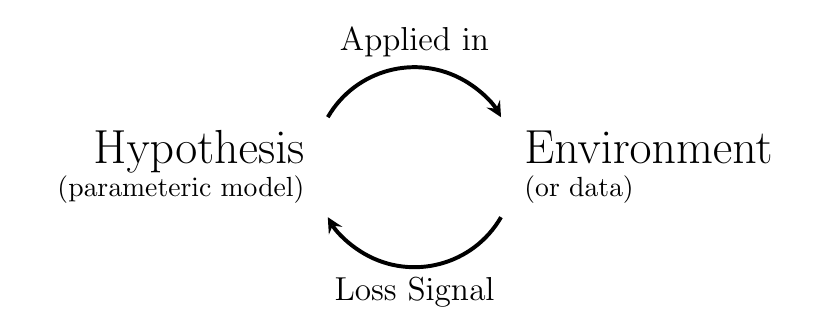
\begin{tikzpicture}[x=1in, y=1in, inner sep=0in, outer sep=0in]

\draw[black, thick, line width=0.5mm, -stealth] ({-0.866 * \arst},{0.5 * \arst}) arc (150:30:\arst);
\draw[black, thick, line width=0.5mm, -stealth] ({0.866 * \arst},{-0.5 * \arst}) arc (-30:-150:\arst);
\node[anchor=west] at ({1.1 * \arst}, 0) {
  \begin{minipage}{100pt}
    {\LARGE Environment} \\
    (or data)
  \end{minipage}
};
\node[anchor=east] at (-{1.1 * \arst}, 0) {
  \begin{minipage}{100pt}
    \raggedleft
    {\LARGE Hypothesis} \\
     (parameteric model)
  \end{minipage}
};

\node[anchor=north] at (0, -{1.1 * \arst}) {
  \begin{minipage}{100pt}
    \centering
    \large
    Loss Signal
  \end{minipage}
};

\node[anchor=south] at (0, {1.1 * \arst}) {
  \begin{minipage}{100pt}
    \centering
    \large
    Applied in
  \end{minipage}
};

\end{tikzpicture}
\end{document}
